\scanpage{19}
% lines 1–2
ce qui n'est autre que la définition (58) explicitée par (59) (en posant $f(x)=y'$).

% lines 2a
% margin note written sideways
\margin{Notons enfin (60) $\overbrace{\operatorname{Tr}\rho_E(\eta')=0}$ (qui exprime que $\rho_E(\eta')$ ``invarie'' $\omega$ (\unsure{et de|admis|idem} $=$ pour $\rho_{E'},\unsure{\widetilde\rho_{\widetilde E}|\rho_{\widetilde E}|\widetilde\rho_E},\rho_{\unsure{\widetilde E'} }\ldots$)}

% lines 2b
% margin note written sideways
\margin{\uline{NB} Faisant $x=y$ dans (52), on trouve \deleted{\unsure{Aussi} \unsure{facilement} \unsure{(quand 2 est} un} $2\varphi(x,\rho_{E'}(\eta')x)=0$, en fait on a même (52 bis) $\varphi(x,\rho_{E'}(\unsure{q'|\eta'|\xi'})\mathbin{.}x)=0$ (se déduit de la précédente, par principe de prolongement \ldots) ; quand $\varphi$ est associée à une forme quadratique, cette formule (52 bis) signifie que l'action de $\mathfrak g=E'$ sur $E$ invarie cette forme quadratique -- c'est plus fort que le fait d'invarier $\varphi$ \ldots}

% lines 3
\figure{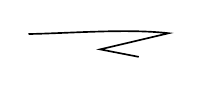
\begin{tikzpicture}[x=1cm,y=1cm]\draw[line width=.6pt] (0,.23) .. controls (.54,.24) and (1.25,.30) .. (1.78,.24) -- (.91,.035) -- (1.4,-.06);\end{tikzpicture}}

% lines 4–7
Reprenons l'exemple de la forme quadratique (21) et la forme $\varphi$ associée (22), d'où la structure d'algèbre de Lie (26) sur $E'$ de base $X=e'_1$, $Y=e'_2$, $H=e'_3$, et

% lines 8
\[
\omega'=-X\wedge H\wedge Y \tag*{(61)}
\]

% lines 9–11
(\inserted{Au lieu de $\omega$} on aurait pu choisir \inserted{\unsure{carrément}} $\omega'=-\omega=X\wedge H\wedge Y$ sans inconvénient, on aurait toujours une structure orthogonale spéciale $(q,\omega')\ \ldots$)

% lines 12–13
Explicitons alors par calcul toutes les opérations précédentes. On posera aussi

% lines 14
\[
\widetilde X=e_2,\quad\widetilde Y=e_1,\quad\widetilde H=e_3 \tag*{(62)}
\]

% lines 15–18
\deleted{or} et quand on regardera $E$ $(\simeq\mathscr O_S^3)$ comme une Algèbre de Lie, nous \unsure{préférerons|préfixerons|préférons} ces notations pour la base, qu'on prendra dans l'ordre

% lines 19
\[
\widetilde X,\ \widetilde H,\ \widetilde Y \tag*{(63)}
\]

% lines 20–22
\[
\text{\deleted{donc}}\quad\omega=\deleted{\unsure{-}}\widetilde X\wedge\widetilde H\wedge\widetilde Y
\quad\text{(\uline{NB} il n'y a pas de signe $-$ ici !)} \tag*{(64)}
\]

% lines 23
On trouve

% lines 24
\[
f(\widetilde X)=X,\ f(\widetilde Y)=Y,\quad f(\widetilde H)=2H \tag*{(65)}
\]

% lines 25
Ici, en vertu de (32)

% lines 26
\[
\Delta=\deleted{\unsure{2}}-2
\]

% lines 27
d'où on trouve

% lines foot
% archive sheet number: 18
